\section{Introduction}
\label{sec:introduction}

Electronic markets emit some of the richest sequential data in any applied domain, and a
large literature reads that data with modern machine learning: deep networks predict
short-horizon price moves from the limit order book \citep{zihao2018deeplob,
briola2024deep, briola2024hlob, sirignano2016deep}, order-flow imbalance is engineered
into ever finer features \citep{bechler2014optimal}, and execution models chase the last
basis point of implementation shortfall \citep{kato2014vwap, curato2014optimal}. The
common working assumption is monotone: a feed with more levels, more history, and a more
faithful reconstruction of the hidden book should let a good learner make better
predictions and, in turn, better decisions. Data vendors price granularity accordingly.

The assumption is rarely tested as a controlled intervention. Most studies vary the
model while holding the information fixed, or improve a forecasting score without asking
what the score buys once a decision policy, a spread, a latency, and a cost intervene.
When forecast quality and decision quality are examined together, the two can come
apart \citep{falezza2026when, raeth2025forecast, anri2026when}, and forecast-evaluation
tools that sweep decision thresholds already warn that a single accuracy number is a
weak surrogate for usefulness \citep{f2017murphy, timo2023evaluating}. What is missing is
a clean, matched measurement on real market data: fix everything the learner is allowed
to exploit except the information itself, and read the effect at the decision.

\begin{figure}[t]
\centering
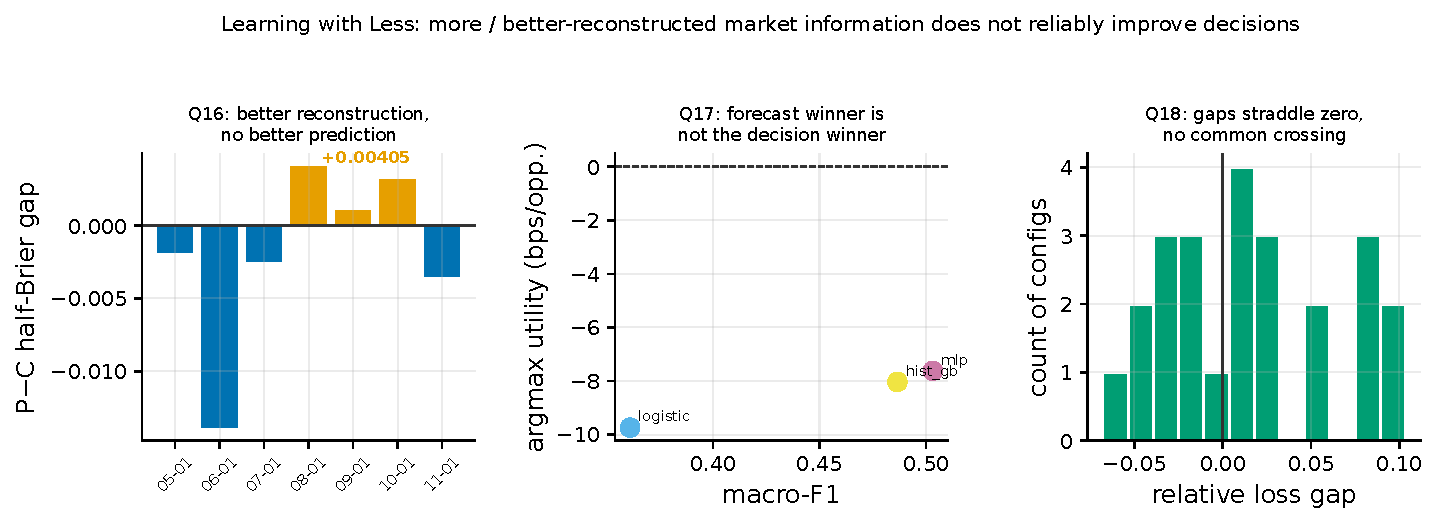
\includegraphics[width=\linewidth]{figures/fig_teaser.pdf}
\caption{\textbf{One instrument, three negative answers.}
We hold the model family, training budget, evaluation dates, and decision policy fixed
and vary only the information the learner sees, on real Hyperliquid data.
\textbf{Left (Q16):} augmenting a coarse predictor with \emph{more accurately
reconstructed} hidden book summaries does not lower prediction loss. On the August
breakout cohort it is $+0.00405$ half-Brier \emph{worse} than the coarse predictor.
\textbf{Center (Q17):} the model that wins on macro-F1 (\texttt{mlp}) is not the model
that wins on decisions. Every learned policy sits below the zero-utility line at
$5$ bps per side.
\textbf{Right (Q18):} the depth/history/delay effect straddles zero across $120$
model$\times$asset$\times$factor configurations, with no common crossing.}
\label{fig:teaser}
\end{figure}

We build that instrument and run it three ways on Hyperliquid perpetual-futures data
(Figure~\ref{fig:teaser}). Each study is a paired comparison in which only the observed
information changes. \textbf{Q16} asks whether reconstructing hidden order-book structure
improves the decision signal: we compare a coarse predictor, a predictor augmented with
reconstructed hidden summaries, and an observed-rich predictor, all trained and scored
identically. \textbf{Q17} asks whether forecast-quality rankings survive translation into
executable decisions: frozen forecasts from several model families pass through fixed
policies under explicit spread, latency, and cost assumptions. \textbf{Q18} asks whether
any fixed book depth, history length, or update delay is universally sufficient: a frozen
factorial varies each axis on matched dates. The headline is that all three answers are
negative, and they agree: better intermediate information does not reliably become better
decisions.

Our contributions are the following.
\begin{itemize}[leftmargin=1.4em]
\item \textbf{A matched information-intervention protocol} for real order-book data that
 fixes model, budget, dates, and policy and varies only the observed information, so the
 effect is read at the decision rather than at a forecasting score
 (Section~\ref{sec:setup}).
\item \textbf{A decision-grade negative for reconstruction (Q16):} across seven monthly
 breakout cohorts every hidden summary is reconstructed more accurately than a frozen
 baseline, yet the reconstruction-augmented predictor is $+0.00405$ half-Brier worse than
 the coarse predictor and $0.01762$ worse than a training-frequency baseline on the
 $691$-event August cohort. Controlled mechanism studies reproduce the same null
 (Section~\ref{sec:q16}).
\item \textbf{A forecast-then-decision reversal audit (Q17):} a multilayer perceptron
 beats logistic regression on macro-F1 by $0.142$ (BTC) and $0.097$ (ETH) while every
 learned policy loses money at $5$ bps per side. $0$ of $8$ protocol contrasts pass the
 joint gate (Section~\ref{sec:q17}).
\item \textbf{A sufficiency factorial (Q18):} no depth, history, or delay setting yields a
 common cross-asset benefit across $120$ fits, and the sign of the effect flips with
 model and asset, so no universal sufficiency threshold exists in this panel
 (Section~\ref{sec:q18}).
\item \textbf{A released, laptop-reproducible programme} of thirty curated experiment
 packages with source certification, provenance, and honest scientific status labels
 (Section~\ref{sec:synthesis}). An anonymized copy of the code, results, and this paper is
 available at \url{https://anonymous.4open.science/r/learning-with-less-C713}.
\end{itemize}

The result is not that information is worthless. It is that its value is conditional,
small, and easily destroyed by the policy and cost layer that any real decision must
cross. We argue this is the more useful thing to measure.
